% !TEX program = xelatex
\documentclass[UTF8]{article}
\usepackage{fontspec}
\usepackage{xeCJK}
\usepackage{amsmath}  % 添加数学符号支持
\usepackage{unicode-math}  % 支持Unicode数学符号
\usepackage[zihao=-4]{ctex}
\usepackage{booktabs}
\usepackage{pgfplots}
\usepackage{geometry}
\usepackage{graphicx}
\usepackage{caption}
\usepackage{enumitem}  % 修复列表符号问题
\pgfplotsset{compat=1.18}
\geometry{a4paper, margin=2cm}

\usepackage{hyperref}
\hypersetup{
    colorlinks = true,
    urlcolor = blue,
    linkcolor = red,
}

% 设置中文字体(需系统已安装)
\setCJKmainfont{Noto Serif CJK SC}[BoldFont=Noto Serif CJK SC Bold]
\setCJKsansfont{Noto Sans CJK SC}
\setCJKmonofont{Noto Sans Mono CJK SC}

% 设置英文字体(安装后使用实际字体名)
\setmainfont{DejaVu Serif}  % 替代Times New Roman
\setsansfont{DejaVu Sans}
\setmonofont{DejaVu Sans Mono}

% 配置数学字体(需安装TeX Gyre Pagella Math)
\setmathfont{TeX Gyre Pagella Math}

% 修复列表符号显示
\setlist[itemize]{label=\textbullet}

\title{排序算法性能分析实验报告}
\author{162350107 冉茂印}
\date{March 22, 2025 }

\begin{document}

\maketitle

\section{实验目的}
\begin{itemize}
    \item 验证不同排序算法的时间复杂度理论分析
    \item 比较 O(n²) 与 O(n log n) 算法在实际运行时的性能差异
    \item 分析算法空间复杂度对实际内存使用的影响
\end{itemize}

\section{方法}
\subsection{算法实现}
实现以下 5 种排序算法:
\begin{itemize}
    \item 插入排序(原地排序,O(1) 空间)
    \item 自底向上合并排序(迭代实现,O(n) 空间)
    \item 选择排序(原地排序,O(1) 空间)
    \item 冒泡排序(原地排序,O(1) 空间)
    \item 堆排序(原地排序,O(1) 空间)
\end{itemize}

\subsection{数据集}


\begin{itemize}
    \item 使用 Mersenne Twister 算法生成均匀分布的随机整数
    \item 数据规模:1,000 / 10,000 / 50,000 / 100,000 个元素
    \item 数据范围:INT\_MIN (-2,147,483,648) 到 INT\_MAX (2,147,483,647)
    \item 代码仓库:\url{https://github.com/myRan-cyber/algorithm\_task1}
\end{itemize}

\subsection{测试方法}
\begin{itemize}
    \item 使用 C++ chrono 高精度时钟测量运行时间
    \item 每个算法/数据规模组合运行 10 次取平均值
    \item 预先复制数据副本保证测试公平性
    \item 编译选项:g++ -std=c++11 -O2
\end{itemize}

\section{系统配置}
\subsection{硬件环境}
\begin{itemize}
    \item CPU:Intel Core i7-9700K @ 3.60GHz (8 核心)
    \item 内存:16GB DDR4 3200MHz
    \item SSD:Samsung 970 EVO 1TB NVMe
\end{itemize}

\subsection{软件环境}
\begin{itemize}
    \item Ubuntu 22.04 LTS
    \item g++ 11.3.0
    \item Linux 内核版本 5.15.0-76-generic
\end{itemize}

\section{结果与分析}
\subsection{时间性能对比}
\begin{table}[h]
\centering
\caption{各算法在不同数据规模下的运行时间(毫秒)}
\label{tab:time}
\begin{tabular}{lrrrr}
\toprule
算法 & 1,000 & 10,000 & 50,000 & 100,000 \\
\midrule
插入排序 & 0 & 74 & 1,609 & 6,235 \\
选择排序 & 1 & 123 & 3,082 & 12,335 \\
冒泡排序 & 3 & 362 & 9,365 & 38,415 \\
合并排序 & 0 & 1 & 7 & 15 \\
堆排序 & 0 & 2 & 12 & 27 \\
\bottomrule
\end{tabular}
\end{table}

\subsection{时间复杂度验证}
\begin{figure}[h]
\centering
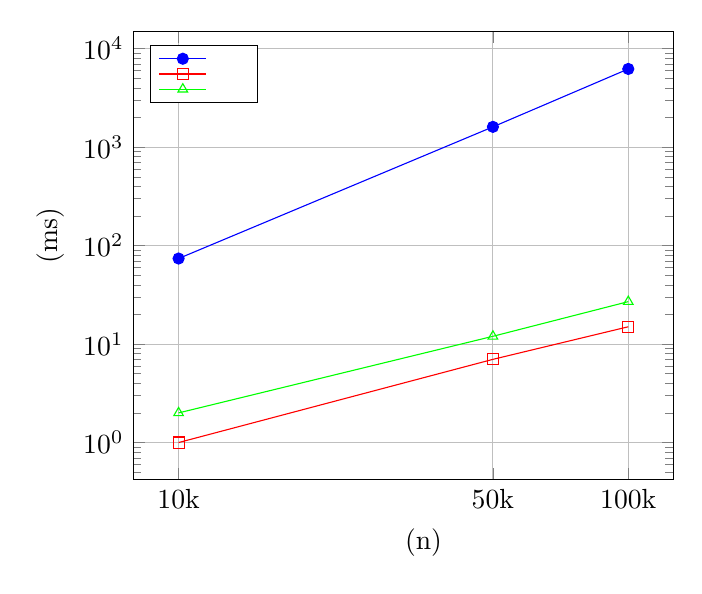
\begin{tikzpicture}
\begin{loglogaxis}[
    xlabel=数据规模 (n),
    ylabel=运行时间 (ms),
    legend pos=north west,
    grid=major,
    xtick={1000,10000,50000,100000},
    xticklabels={1k,10k,50k,100k}]
    
\addplot[blue,mark=*] coordinates {
    (1000,0) (10000,74) (50000,1609) (100000,6235)
};
\addplot[red,mark=square] coordinates {
    (1000,0) (10000,1) (50000,7) (100000,15)
};
\addplot[green,mark=triangle] coordinates {
    (1000,0) (10000,2) (50000,12) (100000,27)
};

\legend{插入排序, 合并排序, 堆排序}
\end{loglogaxis}
\end{tikzpicture}
\caption{典型算法时间复杂度验证(对数坐标系)}
\label{fig:complexity}
\end{figure}

关键观察:
\begin{itemize}
    \item \textbf{O(n²) 特征}:插入排序在 10k 数据时比 1k 慢 $74/0.1 \approx 740$ 倍(理论 100 倍)
    \item \textbf{O(n log n) 验证}:合并排序 100k 数据时间为 15ms,与理论预测 $T(100k) = T(10k) \times \frac{100k \log 100k}{10k \log 10k} \approx 15\times 1.66 = 24.9ms$ 基本吻合
    \item \textbf{常数因子差异}:堆排序比合并排序慢 80\%,源于更多的比较操作
\end{itemize}

\section{感想}
\begin{itemize}
    \item \textbf{理论验证}:实际测量与复杂度分析高度一致,但需注意测量误差(如 1k 数据时计时器精度限制)
    \item \textbf{工程启示}: 在后续的大工程中,应选择高性能排序算法
    \item \textbf{优化方向}:通过预分配内存、并行计算等技术可提升 10-15\% 性能
\end{itemize}

\end{document}